
\section{Signal Model}

This analysis studies the simplified model shown in Figure \ref{fig:feyn}, targeting primarily the decays via Higgs boson.
These are models of \gls{ggm} \cite{Meade:2008wd,Cheung:2007es,Dine:1981gu,AlvarezGaume:1981wy,Nappi:1982hm} 
(already discussed in Section \ref{sec:susybreaking})
or \gls{gmsb} \cite{Dimopoulos:1996vz,Matchev:1999ft} where 
the lightest neutralino is the \gls{nlsp}, that decays promptly to the gravitino ($\gravino$), which is the \gls{lsp}, and 
a \gls{sm} boson. 

\begin{figure}[htbp]
	\centering
	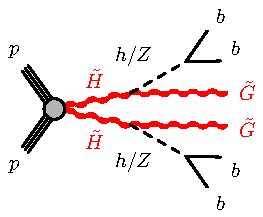
\includegraphics[width=0.35\textwidth]{figures/ewk_prod/varie/N1N1-hhGG-bbbb_Z}
	\caption{Diagram for the simplified model considered in the analysis. The primary interpretation of the analysis is the decay via Higgs bosons, but decays via varied branching ratios to $Z$ bosons are also studied. The production of the \hino\ occurs
via mass-degenerate pairs of charginos or neutralinos, which decay to the \ninoone\ and immeasurably low momentum particles.} 
	\label{fig:feyn}
\end{figure}

As discussed in Section \ref{sec:theo:mssm} \gls{susy} predicts five Higgs bosons. 
Their superpartners (Higgsinos) mix with the superpartners of the electroweak gauge bosons to form charginos and neutralinos.

In models where the the lightest neutralinos and charginos are dominated by the Higgsino component, the four lightest charginos 
and neutralinos are nearly degenerate \cite{Papucci:2011wy,Barbieri:2009ev,Han:2014kaa} and ordered as: $m_{\tilde\chi^0_1}~<~m_{\tilde\chi^\pm_1}~<~m_{\tilde\chi^0_2}$.
These models are particularly interesting because they arise in the limit where $|\mu| < |M_1|, |M_2$|, which is the same limit 
that minimizes the fine tuning problem in the Higgs sector of the \gls{mssm}.

In the case of a Higgsino-like neutralino, the direct production of a \ninoone\ninoone\ pair is suppressed, and the production cross section is dominated by 
\ninoone\ninotwo, \ninoone\chinoonepm, \ninotwo\chinoonepm, and \chinoonep\chinoonem production.
The \ninotwo and \chinoonepm then decay to the \ninoone and soft particles that can not be detected (originating from the 
decay of off-shell W and Z bosons), therefore all of these production processes give practically the same final state as 
\ninoone\ninoone\  pair production. 

Since in this chapter we consider only the case where the lightest neutralino is dominated by the Higgsino component,
we will use interchangeably the notation \ninoone or \hino to indicate it.  
We consider only the case where the lifetime of the \hino is very short and it decays promptly to a Higgs boson or a Z boson and the \gravino;
this is the case when the mass of the mediators of \gls{susy} breaking is relatively small (smaller than $\approx 10^7$ GeV), 
while for higher mediator masses the \gls{nlsp} acquires a finite lifetime, and can pass through the full detector without decaying. 

The analysis described in this thesis targets events where the \gravino is produced with enough transverse momentum to lead to 
sizable \met. This is the case when the Higgsinos have intermediate or high mass.
This search is not sensitive to events where the Higgsino mass is close to the mass of the Higgs boson, and therefore 
the signal events have very little \met and do not fire the \met trigger.
These events are the focus of a dedicated analysis whose results are here briefly discussed in Section \ref{sec:ewk:LM}.


\subsection{Signal cross section}

The signal cross section is computed for the pure Higgsino case, at \gls{nlo} plus \gls{nll} precision, assuming that
\ninoone, \ninotwo and \chinoonepm are degenarate and that all the other \gls{susy} particles decouple \cite{Fuks:2012qx,Fuks:2013vua}.
The nominal cross section and its uncertainty are taken from an envelope of two cross section predictions using different \gls{pdf} sets, 
and it is 3830 $\pm$ 160 fb at $\mhino = 150$ GeV, while it decreases to 1.8 $\pm$ 0.2 fb at $\mhino = 900$ GeV. 

\subsection{Higgsino decay modes}

This search is optimized to target cases where both \hino decay promptly to a Higgs boson and a gravitino with 100\% \gls{br}.
This is not the case in realistic models, where the decays of a short-lived Higgsino in \gls{ggm} scenario 
can be to photon, Z-boson or Higgs boson with 
\gls{br} that depends on the choice of the parameters.
As discussed in Ref. \cite{Meade:2009qv}, the relative width of the three decays of the \ninoone is:

\begin{eqnarray}
\label{eqn:brfhi}
\Gamma(\tilde\chi_1^0\to \tilde G+\gamma)&=& {1\over2}(s_\beta+\eta c_\beta)^2\left({c_Ws_W(M_1-M_2)m_Z\over M_1 M_2}\right)^2 {\cal A} \;,
\nonumber\\
 \Gamma(\tilde\chi_1^0\to \tilde G+Z)&=&{1\over4}(s_\beta+\eta c_\beta)^2\left(1 - \frac{m_Z^2}{m^2_{\tilde{\chi}^0_1}}\right)^4 {\cal A} \;,\\
  \Gamma(\tilde\chi_1^0\to \tilde G+h)&=&{1\over4}(s_\beta-\eta c_\beta)^2\left(1 - \frac{m_h^2}{m^2_{\tilde{\chi}^0_1}}\right)^4 {\cal A} \;. \nonumber
\end{eqnarray}

\noindent In Equation \ref{eqn:brfhi}, {\cal A} is a parameter related to the Higgsino lifetime:
\begin{equation}
\label{eqn:decaylength}
{\cal A} = \frac{m^5_{\tilde{\chi}^0_1}}{16\pi F_0^2} \approx \left(\frac{m_{\tilde{\chi}^0_1}}{100~{\rm GeV}}\right)^5 \left(\frac{100~\rm{TeV}}{\sqrt{F_0}}\right)^4 \frac{1}{0.1~{\rm mm}} \;,
\end{equation}

$\tan \beta$ is the ratio of the up-type to down-type Higgs \glspl{vev}, and $\eta$ represents the relative sign of the coefficients 
of the two \glspl{vev} in the linear combination that constitutes \ninoone. 
The three \glspl{br} for different choices of the parameters are shown in Figure \ref{fig:HiggsinoBR}.

\begin{figure}[h]
	\centering
	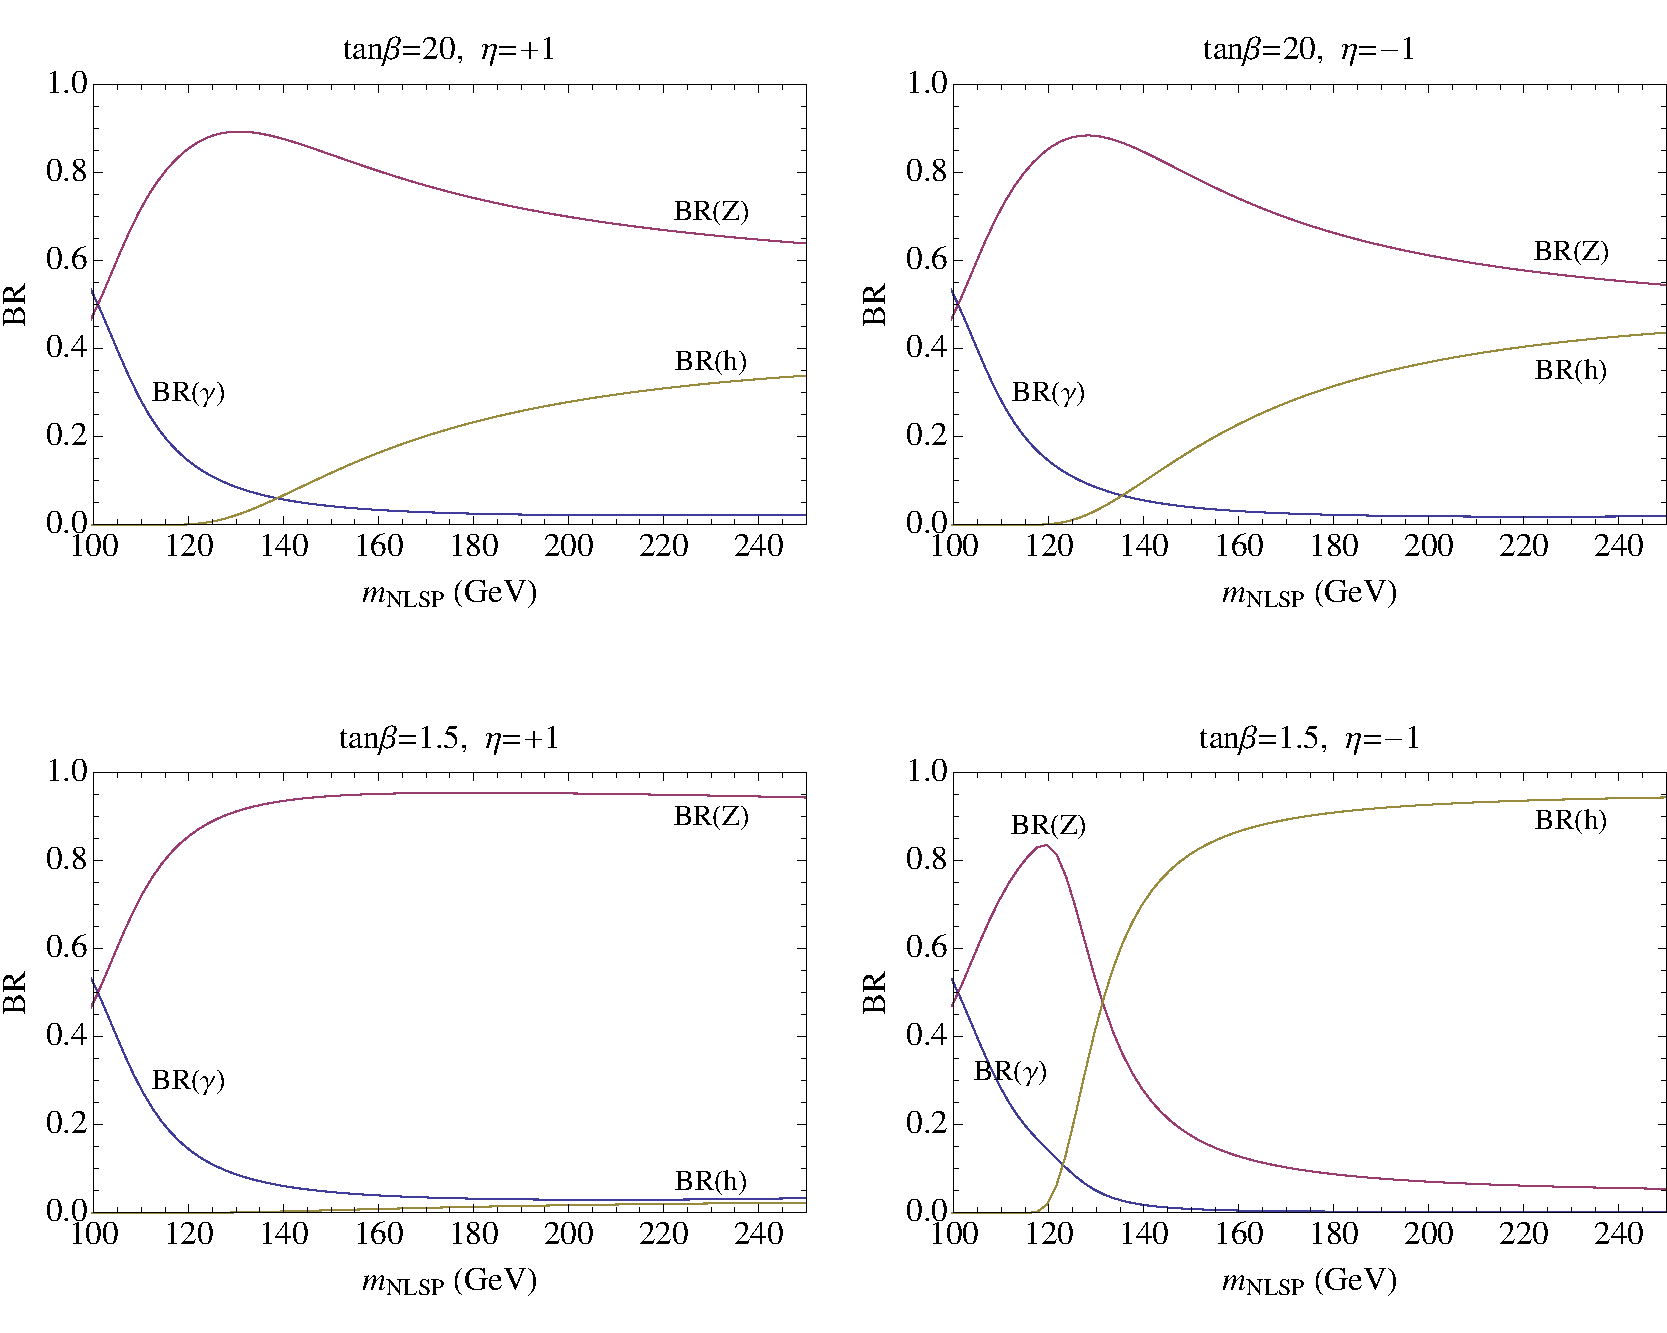
\includegraphics[width=0.95\textwidth]{figures/ewk_prod/varie/BRfracs}
\caption{Branching ratios of the Higgsino NLSP to photons, $Z$'s and Higgses, as a function of $m_{NLSP}$, for $\eta=\pm1$ and $\tan\beta=1.5,\,20$. In all the plots, $M_1=500$ GeV, $M_2=1000$ GeV, and $m_{h^0}=115$ GeV. Figure from Ref. \cite{Meade:2009qv}.}
\label{fig:HiggsinoBR}
\end{figure}

The decay to photon is relevant only for very low m(\hino), where the other decays are kinematically suppressed. 
Once all the kinematic decays are allowed, the \gls{br} is mostly to Z-boson or Higgs boson; 
the assumption of $B(\hino\rightarrow h \tilde{G}) = 100$\%, used to optimize this analysis, is 
realized in the case of relatively low $\tan \beta$ and $\eta = -1$.
Instead for $\tan \beta$ and $\eta = +1$ the dominant decay is to a Z-boson, while for high 
$\tan \beta$ both $B(\hino\rightarrow h \tilde{G})$ and $B(\hino\rightarrow Z \tilde{G})$ tend to 
converge to the same value for high Higgsino mass.
This motivates the interpretation of this analysis as a function of $B(\hino\rightarrow h \tilde{G})$, 
assuming $B(\hino\rightarrow h \tilde{G}) +B(\hino\rightarrow Z \tilde{G}) =1$, presented in Section \ref{sec:ewk:interp}.



%\section{Previous Limits}

